\section{Zweidimensionales Gabor-Wavelet}
\rhead{Zweidimensionales Gabor-Wavelet}

Die Idee des eindimensionalen Gabor-Wavelets wird zuerst als Grundlage genommen. 
Daraus wird dann das zweidimensionale Wavelet abgeleitet und die entstehenden Freiheitsgrade erläutert.

\subsection{Gabor-Wavelet}

Bei der Wavelet-Transformation besteht eine Zeit-Frequenz-Unschärfe.
Diese Unschärfe bewirkt, dass die Auflösung im Zeitbereich umgekehrt proportional zur Auflösung im Frequenzbereich ist.
Das Gabor-Wavelet stellt einen optimalen Kompromiss aus Zeit-und Frequenzauflösung dar.
Die Anwendung des Wavelets minimiert dabei das Produkt der Standardabweichungen im Zeit- und Frequenzbereich \cite{paper:communication}.

Ein solches Gabor-Wavelet besteht aus einer komplexen Schwingung, welche mit einer Gauss-Funktion gefenstert ist.
Diese Fensterung bewirkt eine exponentielle Abnahme der Schwingungsamplitude.
Daraus ergibt die Formel
\begin{equation}\label{eq:1d_gabor}
G(x)= e^{-\frac{(x-x_{0})^{2}}{\sigma^{2}}} e^{i\xi_{0}x}.
\end{equation}

Der Parameter $\sigma$ beschreibt die Standardabweichung der Gauss-Funktion und $\xi_{0}$ die Frequenz der komplexen Schwingung. 
Die Konstante $x_0$ bestimmt die Position des Wavelets.
Die komplexe Schwingung besteht aus einem Sinus- und einem  Kosinus-Anteil. 
Ein Beispiel eines Sinus-Gabor-Wavelet wird in Abbildung \ref{fig:gabor1d} gezeigt.

\begin{figure}
	\centering
	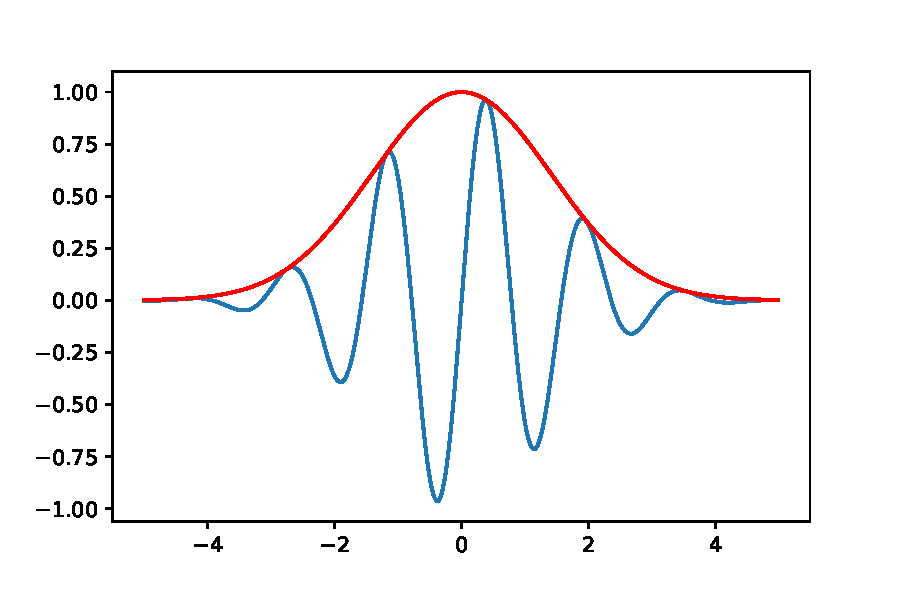
\includegraphics[width=0.7\linewidth]{./papers/visuell/images/gabor_1d}
	\caption{Beispiel eines Sinus-Gabor-Wavelets}
	\label{fig:gabor1d}
\end{figure}


\subsection{Erweiterung auf zwei Dimensionen}\label{subsec:2D}

Um ein solches Wavelet auf ein Bild anwenden zu können ist es notwendig, dieses auf zwei Dimensionen zu erweitern.
Als erstes erweitern wir die komplexe Schwingung aus \ref{eq:1d_gabor} auf eine zweidimensionale, ebene Schwingung.
Wir erhalten
\begin{equation}\label{eq:2d_schwingung}
P_1(x,y)= e^{i(\xi_{0}x+\nu_{0}y)}.
\end{equation}
Diese Schwingung kann man sich als ebene Welle vorstellen, welche abhängig von $\xi_0$ und $\nu_0$ in eine bestimmte Richtung zeigt (vgl. Abbildung \ref{fig:planarwave}).

Als nächsten Schritt erweitern wir die Gauss-Funkion auf eine elliptische, zweidimensionale Gauss-Funktion der Form
\begin{equation}\label{eq:2d_gauss}
P_2(x,y)=e^{-(\frac{(x-x_{0})^{2}}{\sigma^{2}}+\frac{(y-y_{0})^{2}}{\beta^{2}})}.
\end{equation}
Eine elliptische Gauss-Funktion erzeugt Niveaulinien, welche die Form einer Ellipse haben.
Die Standardabweichungen in $x$-, bzw. $y$-Richtung $\sigma$ resp. $\beta$ bestimmen die Ausrichtung und Grösse der Ellipse.
Ein Beispiel einer elliptischen Gauss-Funktion ist in Abbildung \ref{fig:2d_gauss} dargestellt.

Aus den Gleichungen \ref{eq:2d_schwingung} und \ref{eq:2d_gauss} lässt sich die Formel für das zweidimensionale Gabor-Wavelet bilden:
\begin{equation}\label{eq:2dgabor1}
G(x,y)= e^{-(\frac{(x-x_{0})^{2}}{\sigma^{2}}+\frac{(y-y_{0})^{2}}{\beta^{2}})}
e^{i(\xi_{0}x+\nu_{0}y)}.
\end{equation}

\begin{figure}
	\centering
	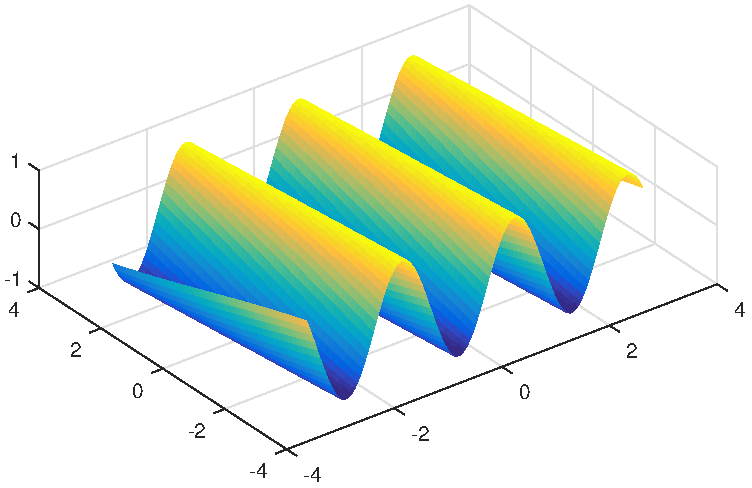
\includegraphics[width=0.7\linewidth]{./papers/visuell/images/planarwave.pdf}
	\caption{Beispiel einer ebenen Schwingung}
	\label{fig:planarwave}
\end{figure}

\begin{figure}
	\centering
	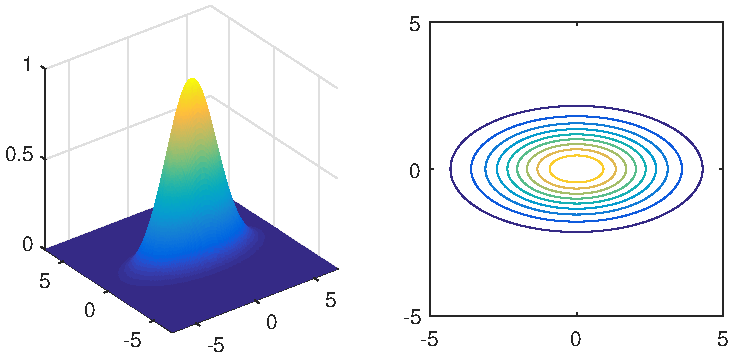
\includegraphics[width=0.7\linewidth]{./papers/visuell/images/2d_gauss.pdf}
	\caption{Beispiel einer elliptischen Gauss-Funktion, links eine dreidimensionale Ansicht, rechts ein Plot der Niveaulinien.}
	\label{fig:2d_gauss}
\end{figure}

Dieses zweidimensionale Wavelet wollen wir mit Hilfe eines neuen Parameters $\theta$ in beliebige Richtungen ausrichten können.
Eine Veränderung von $\theta$ soll also eine Drehung der Wellenfront und der elliptischen Gauss-Funktion bewirken.
Dies bedeutet, dass die Ellipsenachsen (vgl. Abbildung \ref{fig:2d_gauss}) nicht mit den Koordinatenachsen übereinstimmen müssen. 
Um dieses Verhalten zu erreichen führen wir die neuen Variablen $x'=x\cos(\theta)+y\sin(\theta)$ und $y'=-x\sin(\theta)+y\cos(\theta)$ ein.
Diese Formulierung stellt eine Drehmatrix der Art
\begin{equation}
\begin{pmatrix}
x' \\
y'
\end{pmatrix}
=
\begin{pmatrix}
\cos(\theta) & \sin(\theta) \\
-\sin(\theta) & \cos(\theta)
\end{pmatrix}
\begin{pmatrix}
x \\
y
\end{pmatrix}
\end{equation}
dar.
Die Gleichung \ref{eq:2dgabor1} verändern wir so, dass $x'$ und $y'$ eingesetzt werden können.
Ausserdem sind die Parameter ($\sigma$, $\beta$, $\xi$, $\nu$) dieser Formel unhandlich und es ist nicht offensichtlich was eine Änderung derselben bewirkt.
Also ersetzen wir diese durch neue Parameter und erhalten 
\begin{equation}
G(x,y)=e^{-\frac{x'^{2}+\gamma^{2}y'^{2}}{2\sigma^{2}}}
e^{i(2\pi\frac{x'}{\lambda} + \phi)}.
\end{equation} 
Der Parameter $\gamma$ beschreibt das Verhältnis der Streckung in $x$- und $y$-Richtung.
Diese Streckung der elliptischen Gauss-Funktion bestimmt, ob das Wavelet eher rund oder länglich ist.
Die Standardabweichung der Gauss-Funktion, welche mit der Schwingung multipliziert wird, ist als Parameter $\sigma$ definiert.
Grösseres $\sigma$ bewirkt ein breiteres Wavelet.
Die komplexe Schwingung wird durch die Wellenlänge $\lambda$ und die Phase $\phi$ definiert.
Eine Phasenverschiebung scheint keinen klaren Nutzen zu haben und deshalb  wird für den weiteren Verlauf dieses Papers $\phi=0$ gesetzt.
Der Parameter $\theta$ definiert nun die Ausrichtung der komplexen Schwingung.
Eine Änderung von $\theta$  bewirkt somit eine Drehung der Wellenfronten.

Wie sich Gabor-Wavelets in Abhängigkeit dieser Parameter verhalten zeigt Abbildung \ref{fig:kernels}.
Vier unabhängige Freiheitsgrade (Parameter) sind zu viel um einen guten Überblick zu behalten.
Aus diesem Grund werden im weiteren Verlauf dieses Papers die Parameter der Gauss-Funktion $\sigma$ und $\gamma$ fixiert und nur noch die anderen beiden Parameter verändert.

\begin{figure}
	\centering
	\subfigure[Parameter der Gauss-Funktion $\gamma$ und $\sigma$ werden verändert]
	{\label{fig:kernels_a}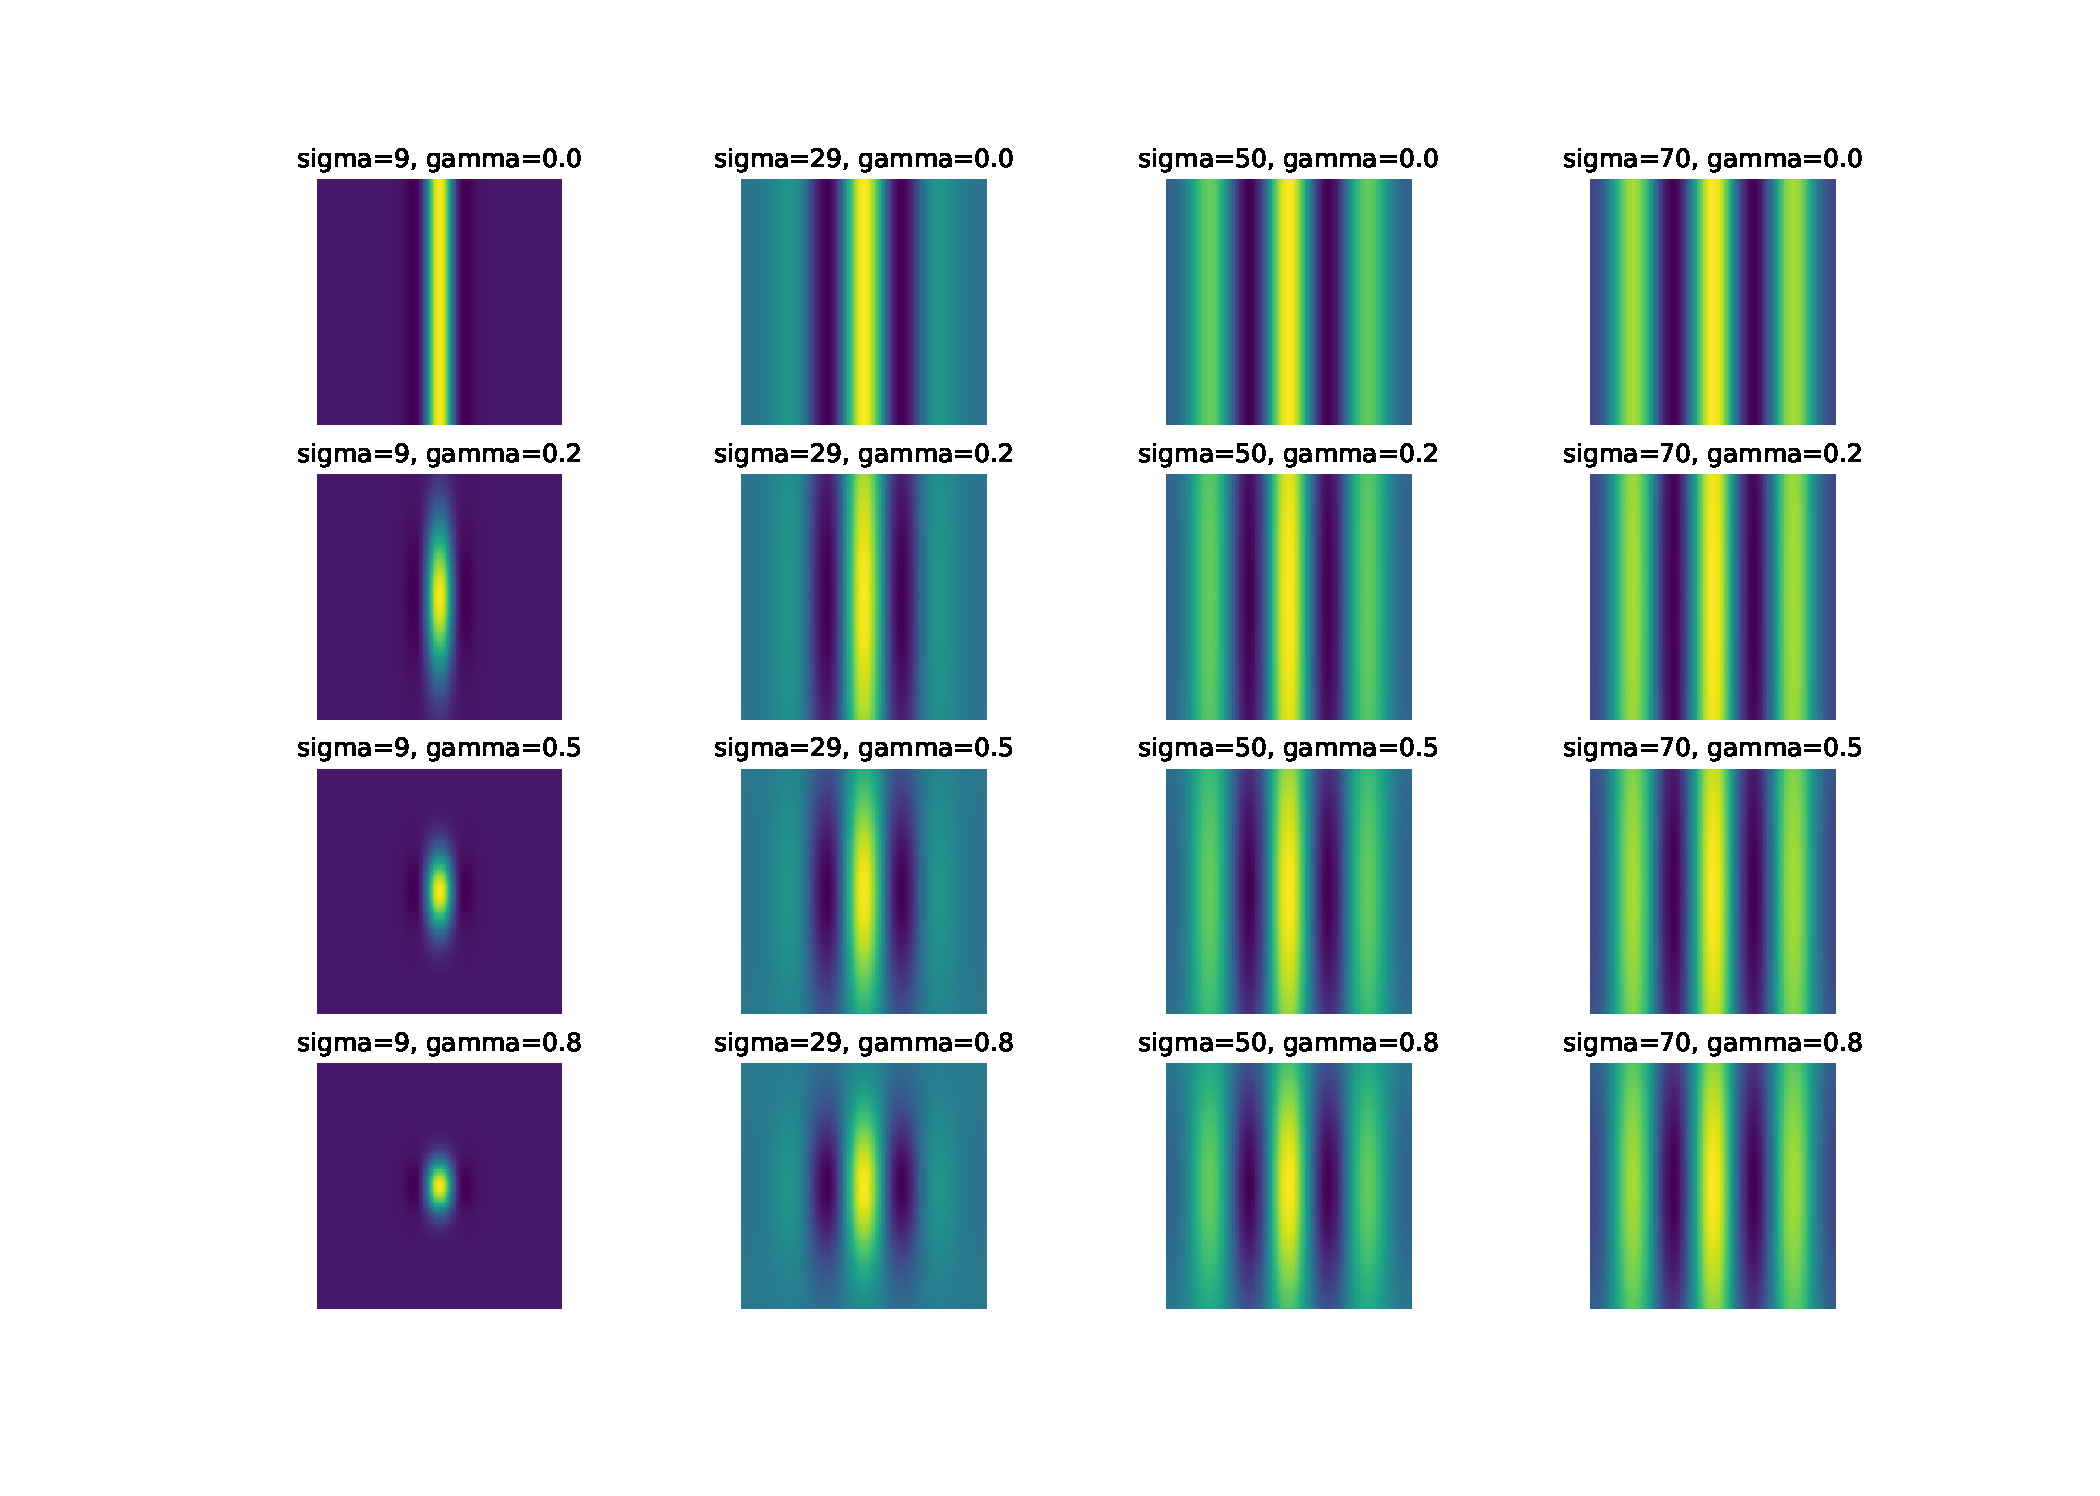
\includegraphics[width=0.8\linewidth, trim=0 60 0 60, clip ]{./papers/visuell/images/kernels_sigma_gamma.pdf}}
	
	\subfigure[Wellenlänge der Schwingung $\lambda$ und Ausrichtung $\theta$ werden verändert]
	{\label{fig:kernels_b}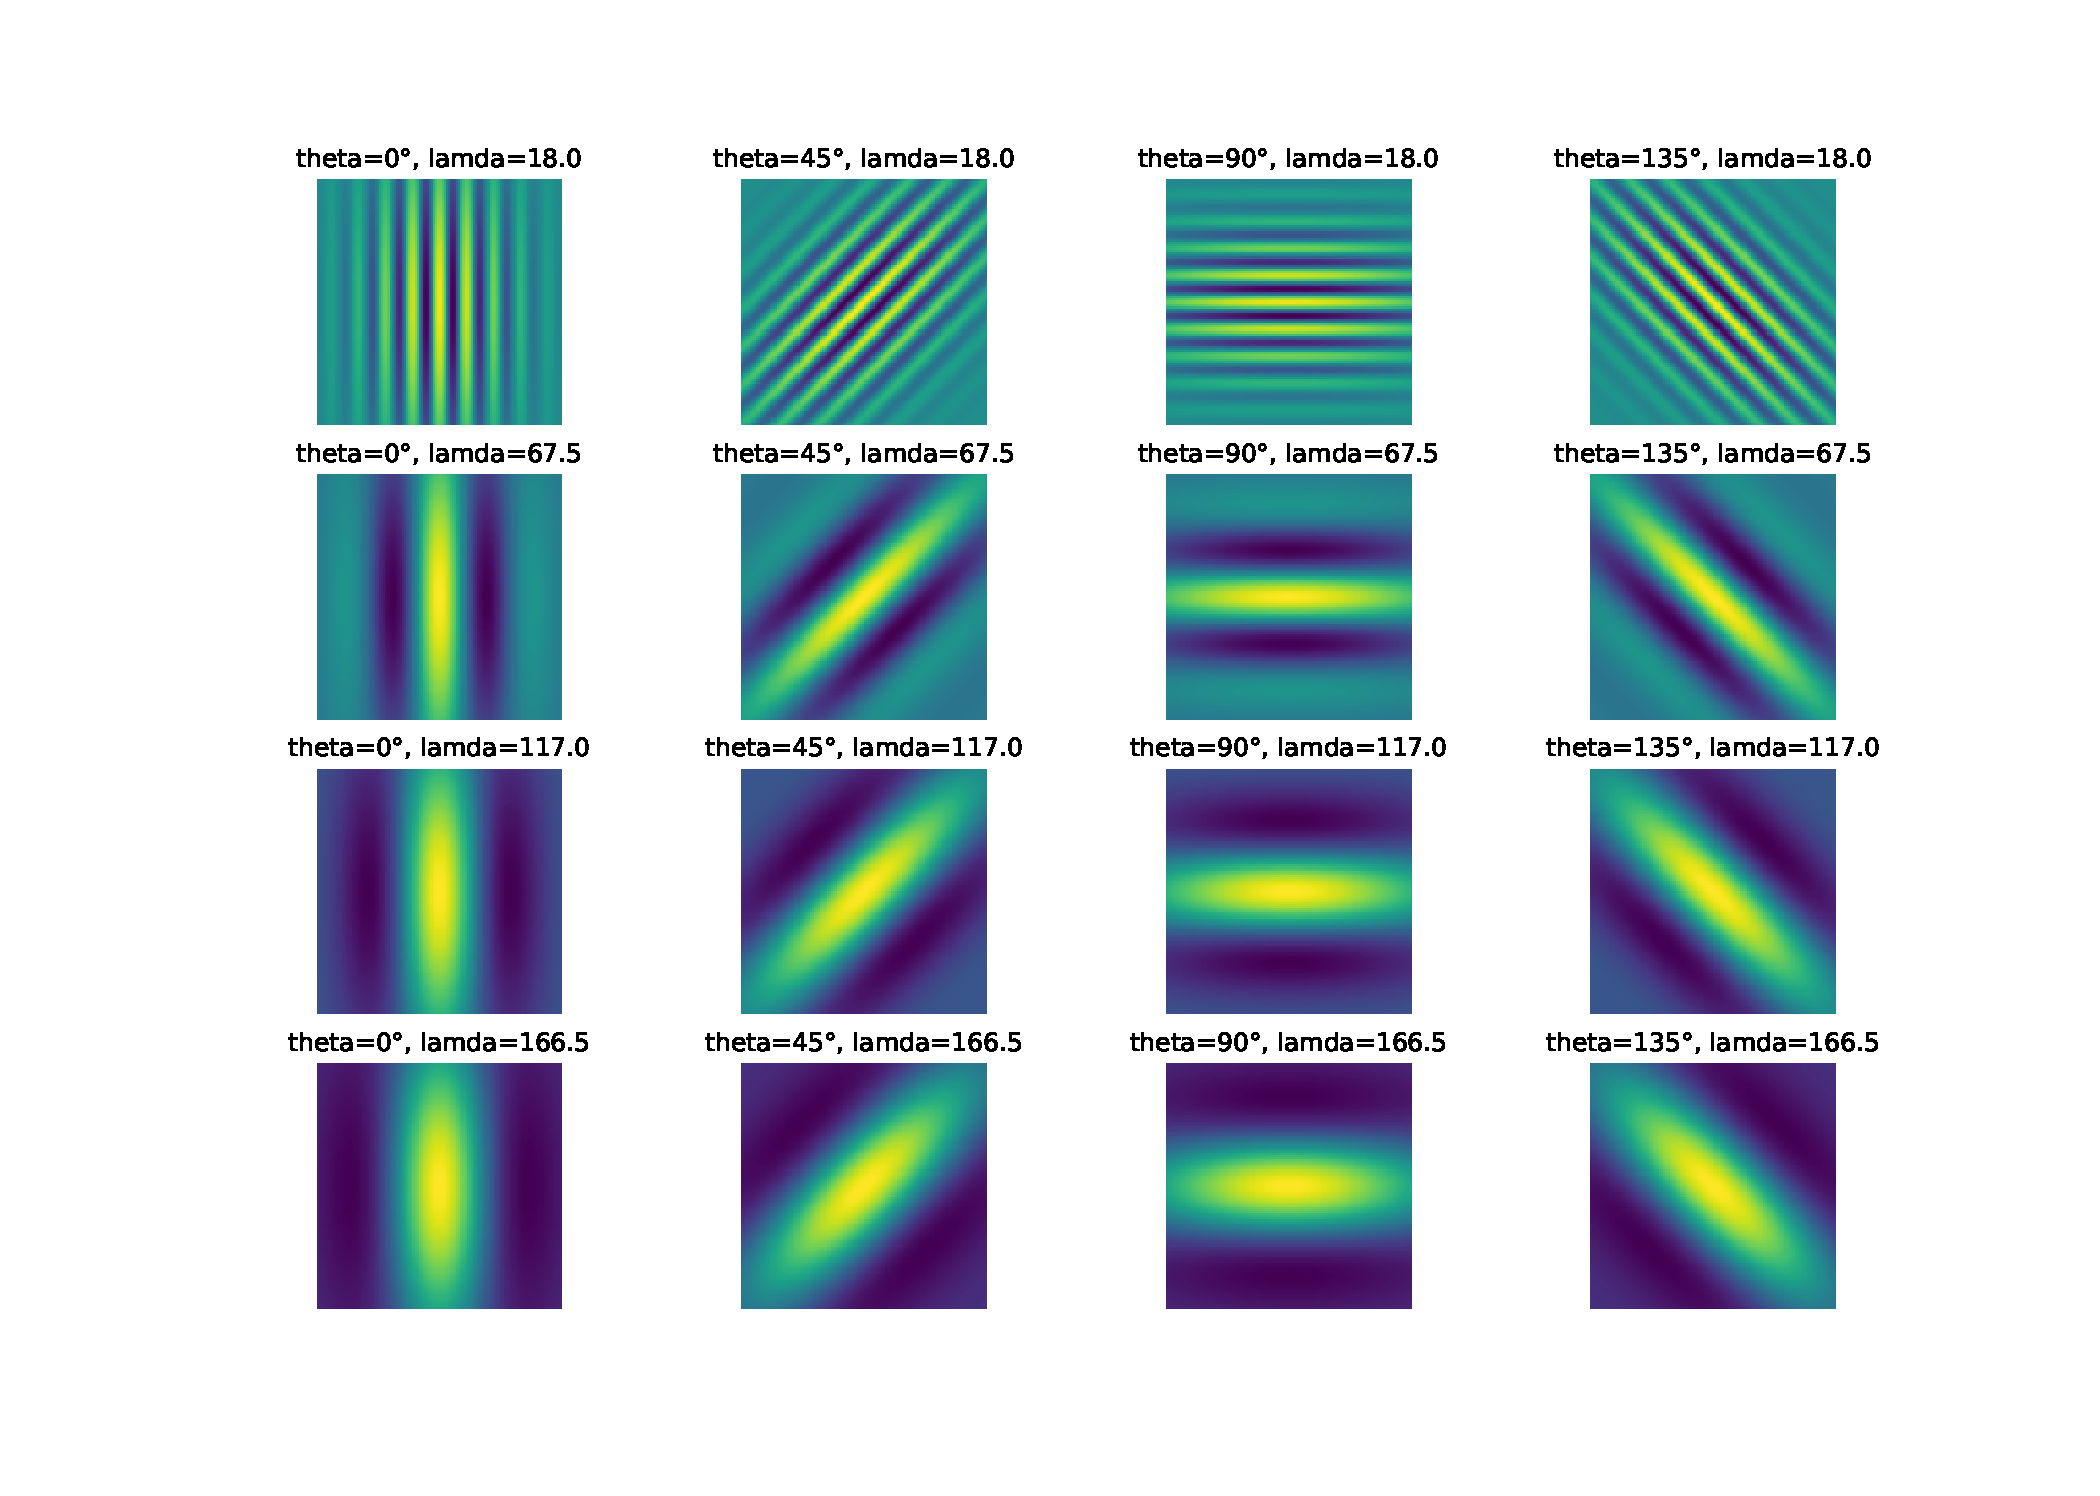
\includegraphics[width=0.8\linewidth, trim=0 60 0 60, clip ]{./papers/visuell/images/kernels_theta_lambda.pdf}}
	
	\caption{Abhängigkeit des Gabor-Wavelets von den Parametern.}
	\label{fig:kernels}
\end{figure}
